\documentclass[11pt]{article}
\usepackage[utf8]{inputenc}
\usepackage[left=2.5cm, top=2cm, right=2cm, bottom=2.5cm]{geometry}
\usepackage{graphicx}
\usepackage{latexsym}
\usepackage{algorithm}
\usepackage{algorithmic}
\usepackage{minted}
\usepackage{caption}

%opening
\title{Lab 0 Report}
\author{Andrés Calderón}

\begin{document}

\maketitle

\section{Introduction}
In this report, two algorithms for sorting arrays of integers, as studied in class, are implemented and analyzed. These algorithms are Insertion-sort and Merge-sort. Once both algorithms were implemented, they were subjected to an empirical analysis to compare their response times and verify the asymptotic analysis illustrated in class. Finally, some observations found during the development of this report are discussed.

\section{Algorithm Implementation}
For the implementation of the algorithms, the pseudocodes studied in class were followed, and the coding was carried out in the Python programming language. Below, we present the pseudocodes and implementations for each algorithm.

\subsection{Insertion-sort}
The pseudocode on which the implementation was based can be seen in Algorithm \ref{alg:insertion}, and the source code of the implementation is presented in Figure \ref{cod:insertion}.

\begin{algorithm}
    \caption{Insertion-sort pseudocode.}
    \begin{algorithmic}[1]
        \STATE \textsc{Insertion-sort}$(A, n)$ \hspace{5mm} $\rhd A[1 \ldots n]$
        \STATE \hspace{1em} \textbf{for} $j \leftarrow 2$ \textbf{to} $n$ \textbf{do}
        \STATE \hspace{2em} $key \leftarrow A[j]$
        \STATE \hspace{2em} $i \leftarrow j - 1$
        \STATE \hspace{2em} \textbf{while} $i > 0$ \textbf{and} $A[i] > key$ \textbf{do}
        \STATE \hspace{3em} $A[i + 1] \leftarrow A[i]$
        \STATE \hspace{3em} $i \leftarrow i - 1$
        \STATE \hspace{2em} $A[i + 1] \leftarrow key$
    \end{algorithmic}
    \label{alg:insertion}
\end{algorithm}

\inputminted[linenos]{python}{insertion_sort.py}
\captionof{figure}{"Implementation of Insertion-sort in Python 3".}\label{cod:insertion}

\subsection{Merge-sort}
Similarly, the pseudocode of Algorithm \ref{alg:merge} was followed for the implementation shown in Figure \ref{cod:merge}.

\begin{algorithm}
    \caption{Merge-sort pseudocode.}
    \begin{algorithmic}[1]
        \STATE \textsc{Merge-sort}$(A, n)$ \hspace{5mm} $\rhd A[1 \ldots n]$
        \STATE \hspace{1em} \textbf{if} $n = 1$, done.
        \STATE \hspace{1em} Recursively sort $A[ 1 \ldots \lceil \frac{n}{2} \rceil ]$ and $A[ \lceil \frac{n}{2} \rceil + 1 \ldots n ]$
        \STATE \hspace{1em} \textsc{Merge} the 2 sorted list.
    \end{algorithmic}
    \label{alg:merge}
\end{algorithm}

\inputminted[linenos]{python}{merge_sort.py}
\captionof{figure}{"Implementation of Merge-sort in Python 3."}\label{cod:merge}

\section{Experiments}
To empirically analyze the performance of the implementations \ref{cod:insertion} and \ref{cod:merge}, the following subroutine was implemented to generate an array of a specified number of integers. The size of the array is passed to the subroutine as the parameter $n$. Figure \ref{cod:array} shows the implementation of this subroutine.

Along with the implementations of both algorithms and the random array generator, a script was programmed to run a series of 5 tests that recorded the execution time of each implementation under different array sizes. The analysis focused on arrays ranging in size from 1000 to 20000 integers. The results were analyzed using the R programming language, where we aggregate the data and compute the average execution time for each case.  Finally, a graph was generated to visually compare the performance of the two algorithms. Figure \ref{fig:sort} illustrates the findings.

\inputminted[linenos]{python}{array_generator.py}
\captionof{figure}{"Implementation of a random array generator in Python 3".}\label{cod:array}

\begin{figure}[t]
    \centering
    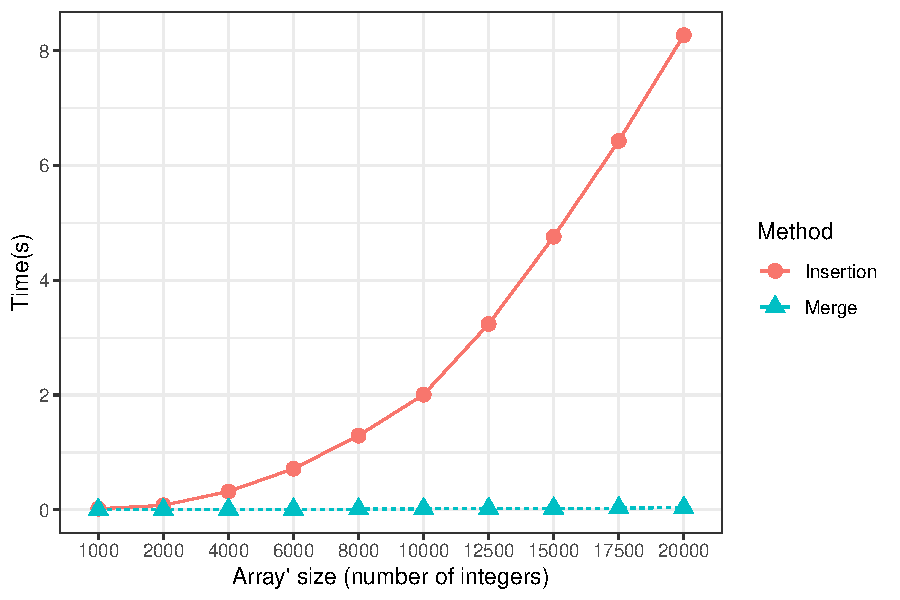
\includegraphics[width=0.7\textwidth]{sort}
    \caption{"Performance of the analyzed algorithms under various array sizes."}
    \label{fig:sort}
\end{figure}

\section{Conclusion}
It is clear that the implementation of Merge-sort has a much better performance than that of Insertion-sort. The response times of Insertion-sort clearly exhibit its quadratic performance, as seen in class ($O(n^2)$). However, the behavior of Merge-sort, under the analyzed array sizes, gives the illusion of constant performance ($O(1)$) instead of logarithmic ($O(n \log n)$). It seems that the implementation would need to be tested with much larger array sizes to observe this expected trend.

\end{document}
